\documentclass{article}


% if you need to pass options to natbib, use, e.g.:
%     \PassOptionsToPackage{numbers, compress}{natbib}
% before loading neurips_2025

\PassOptionsToPackage{numbers, sort, compress}{natbib}

% ready for submission
\usepackage{neurips_2025}


%\bibliographystyle{abbrvnat}
\bibliographystyle{unsrtnat}


\usepackage[pdftex]{graphicx}
\usepackage{amsmath}
% to compile a preprint version, e.g., for submission to arXiv, add add the
% [preprint] option:
%\usepackage[preprint]{neurips_2025}


% to compile a camera-ready version, add the [final] option, e.g.:
%     \usepackage[final]{neurips_2025}


% to avoid loading the natbib package, add option nonatbib:
%    \usepackage[nonatbib]{neurips_2025}


\usepackage[utf8]{inputenc} % allow utf-8 input
\usepackage[T1]{fontenc}    % use 8-bit T1 fonts
\usepackage{hyperref}       % hyperlinks
\usepackage{url}            % simple URL typesetting
\usepackage{booktabs}       % professional-quality tables
\usepackage{amsfonts}       % blackboard math symbols
\usepackage{nicefrac}       % compact symbols for 1/2, etc.
\usepackage{microtype}      % microtypography
\usepackage{xcolor}         % colors

\newcommand\reynotes[1]{\textcolor{purple}{#1}}

%\title{SmokeViz: Using Pseudo-Labels to Develop a Human-Labeled Deep Learning Dataset of Wildfire Smoke Plumes in Satellite Imagery}
\title{SmokeViz: A Large-Scale Satellite Dataset for Wildfire Smoke Detection and Segmentation}


% The \author macro works with any number of authors. There are two commands
% used to separate the names and addresses of multiple authors: \And and \AND.
%
% Using \And between authors leaves it to LaTeX to determine where to break the
% lines. Using \AND forces a line break at that point. So, if LaTeX puts 3 of 4
% authors names on the first line, and the last on the second line, try using
% \AND instead of \And before the third author name.


\author{%
  Rey Koki\\%\thanks{rey.koki@colorado.edu} \\
  Department of Computer Science\\
  University of Colorado Boulder\\
  Boulder, Colorado 80303\\
  \texttt{rey.koki@colorado.edu} \\
  % examples of more authors
  % \And
  % Coauthor \\
  % Affiliation \\
  % Address \\
  % \texttt{email} \\
  % \AND
  % Coauthor \\
  % Affiliation \\
  % Address \\
  % \texttt{email} \\
  % \And
  % Coauthor \\
  % Affiliation \\
  % Address \\
  % \texttt{email} \\
  % \And
  % Coauthor \\
  % Affiliation \\
  % Address \\
  % \texttt{email} \\
}


\begin{document}






\appendix

\section{Supplementary Material}

\subsection{Original Data and Software Licenses}

The HMS Smoke product does not have a license attached to it. For GOES imagery, NOAA states "There are no restrictions on the use of this data" and does not provide a license. Pytroll is distributed under the GNU General Public License v3.0 license and Segmentation Models Pytorch is distributed under the MIT License.


\subsection{Satellite and Band Choice}

\begin{figure}[!htb]
    \centering
    \includegraphics[width=\linewidth]{figures/G17_s20221371250321_35.61_-105.01_36.png}
    \caption{GOES-West better}\label{G16_vs_G17}
\end{figure}


\begin{figure}[!htb]
    \centering
    \includegraphics[width=\linewidth]{figures/G16_s20221550056176_33_-106_all_band.png}
    \caption{All 16 GOES bands}\label{all_bands}
\end{figure}

\subsection{Statistical Visualizations for SmokeViz Dataset}

%Figures \ref{count_per_yr}, \ref{count_per_month}, \ref{count_per_state}, \ref{count_per_country} provide some statistical analysis on \(\mathcal{D}_p\)
Figures \ref{count_per_yr}-\ref{count_per_country} provide some statistical analysis on the SmokeViz dataset. As seen in figure \ref{count_per_yr}, we see the highest number of samples for the year 2020 that showed a high volume of available annotations that year likely due to the large number of wildfires \cite{fires2020} during 2020. The peak for number of samples shown in figure \ref{count_per_month} is March and April, coming right before the typical wildfire season that usually goes from late Spring through Fall. This may be due to the increase in prescribed agricultural burns before plants emerge from winter dormancy \cite{ag_fire}. The HMS analysts do not distinguish between planned or uncontrolled fire, so many of the annotations represent small agricultural burns along with wildfires. If a SmokeViz user desired to only have wildfires represented, they could filter out any fires that are less than one day since controlled agricultural burns tend to be shorter in timespan.

As shown in figure \ref{count_per_state}, the states with the highest number of samples are California, Georgia and Florida. The high frequency in fires in the Southeast may be due to the aforemetioned prescirbed agricultural burns. Analysts are looking not only at the United States, but also Canada and Mexico, figure \ref{count_per_country} shows a breakdown of the number of samples that originate from each country.


\begin{figure}[!htb]
    \parbox{\textwidth}{
      \parbox{0.49\textwidth}{
        \centering
        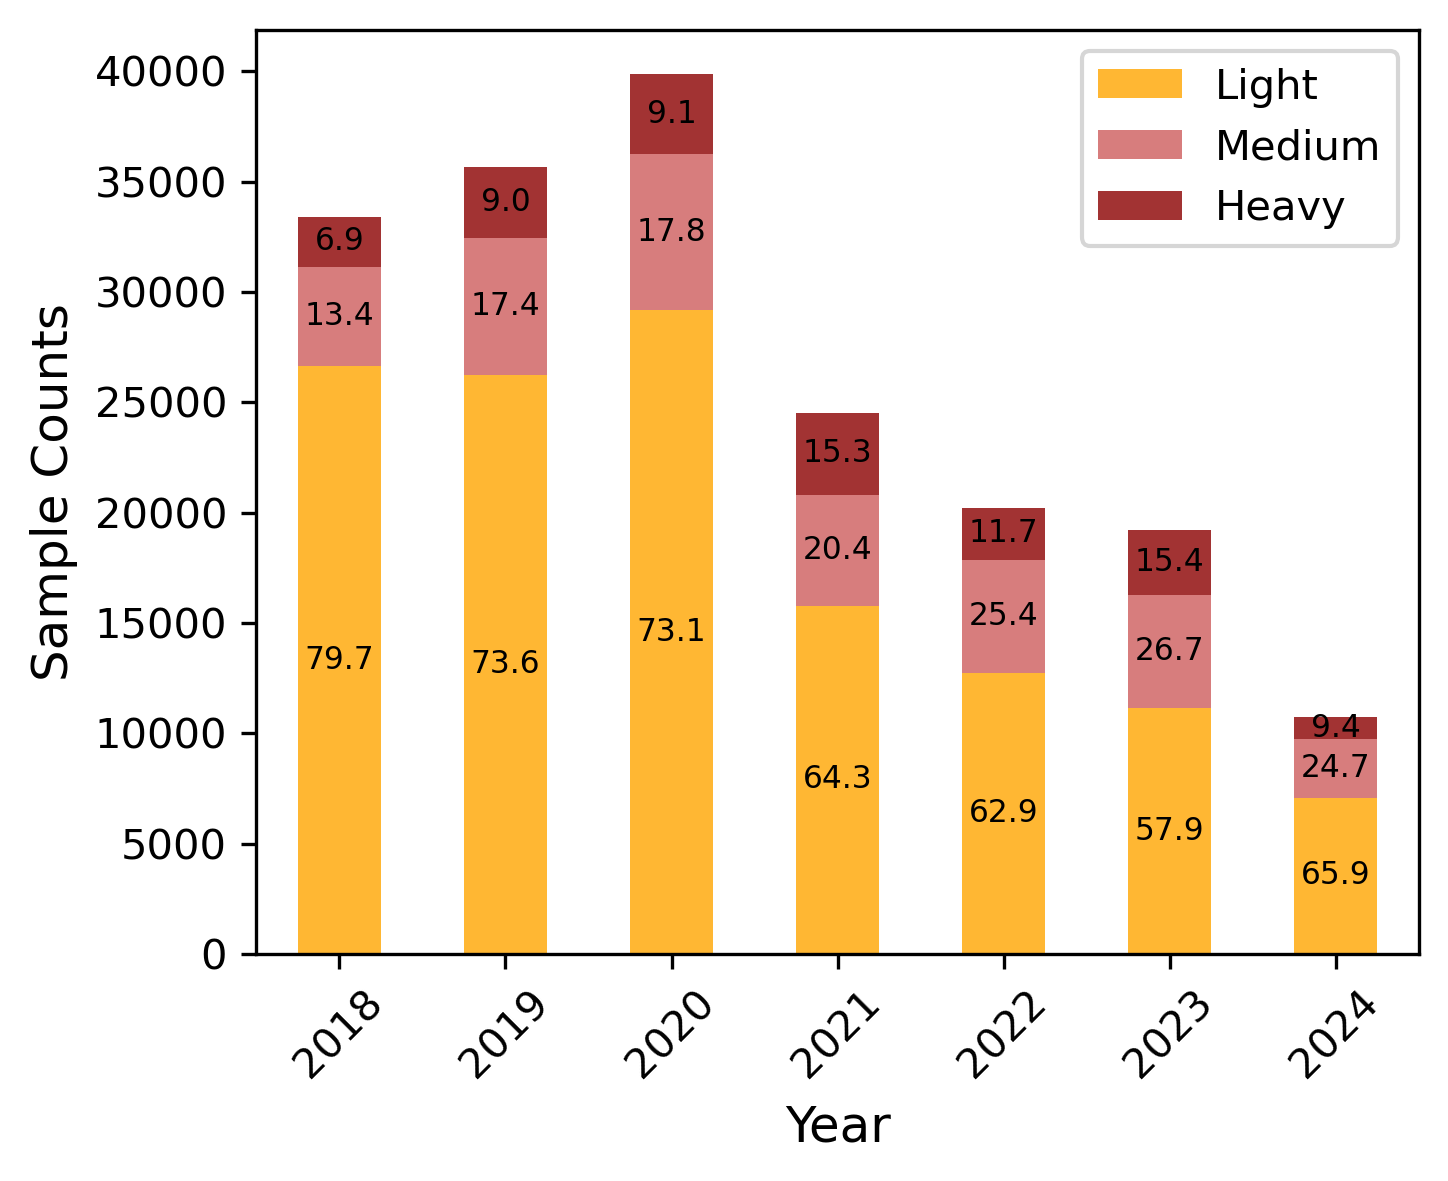
\includegraphics[width=0.49\textwidth]{stat_figs/sample_count_per_yr_percentages.png}
        \caption{Sample count per year for the SmokeViz dataset broken up by smoke density with percent of each density reported within the column.}
        \label{count_per_yr}
      }
    \hspace{0.01\textwidth}
      \parbox{0.49\textwidth}{
        \centering
        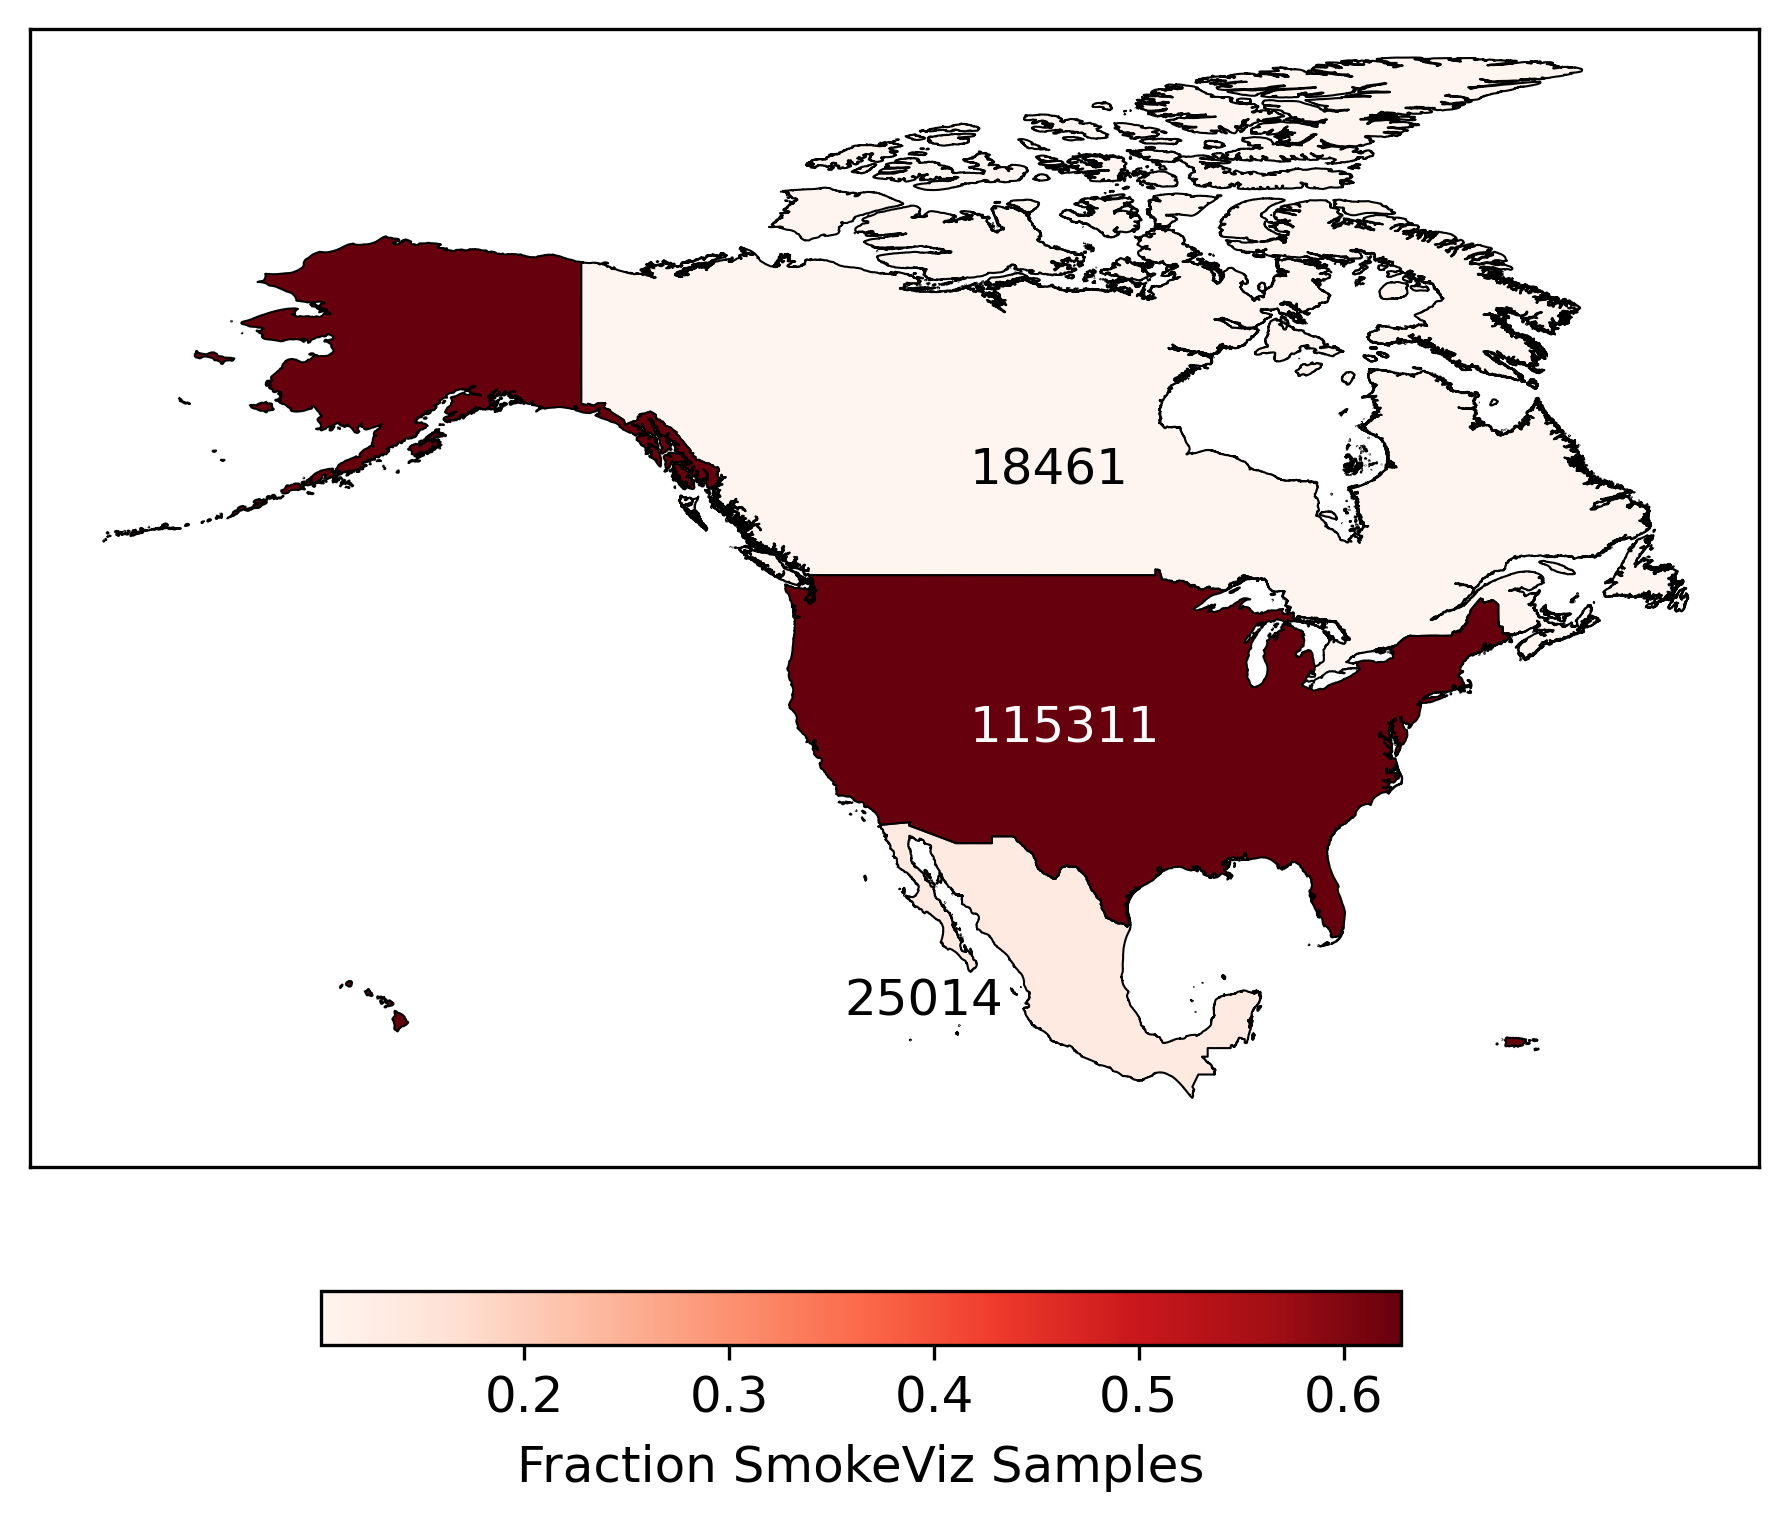
\includegraphics[width=0.49\textwidth]{stat_figs/sample_percent_country.png}
        \caption{Fraction of samples where the center pixel is within the bounds of each country. The counts per country are Canada: 18461, USA: 115,311 and Mexico: 25,014, 24,886 samples have center pixels over other countries/oceans.}
        \label{count_per_country}
      }
    }
\end{figure}

\begin{figure}[!htb]
    \centering
    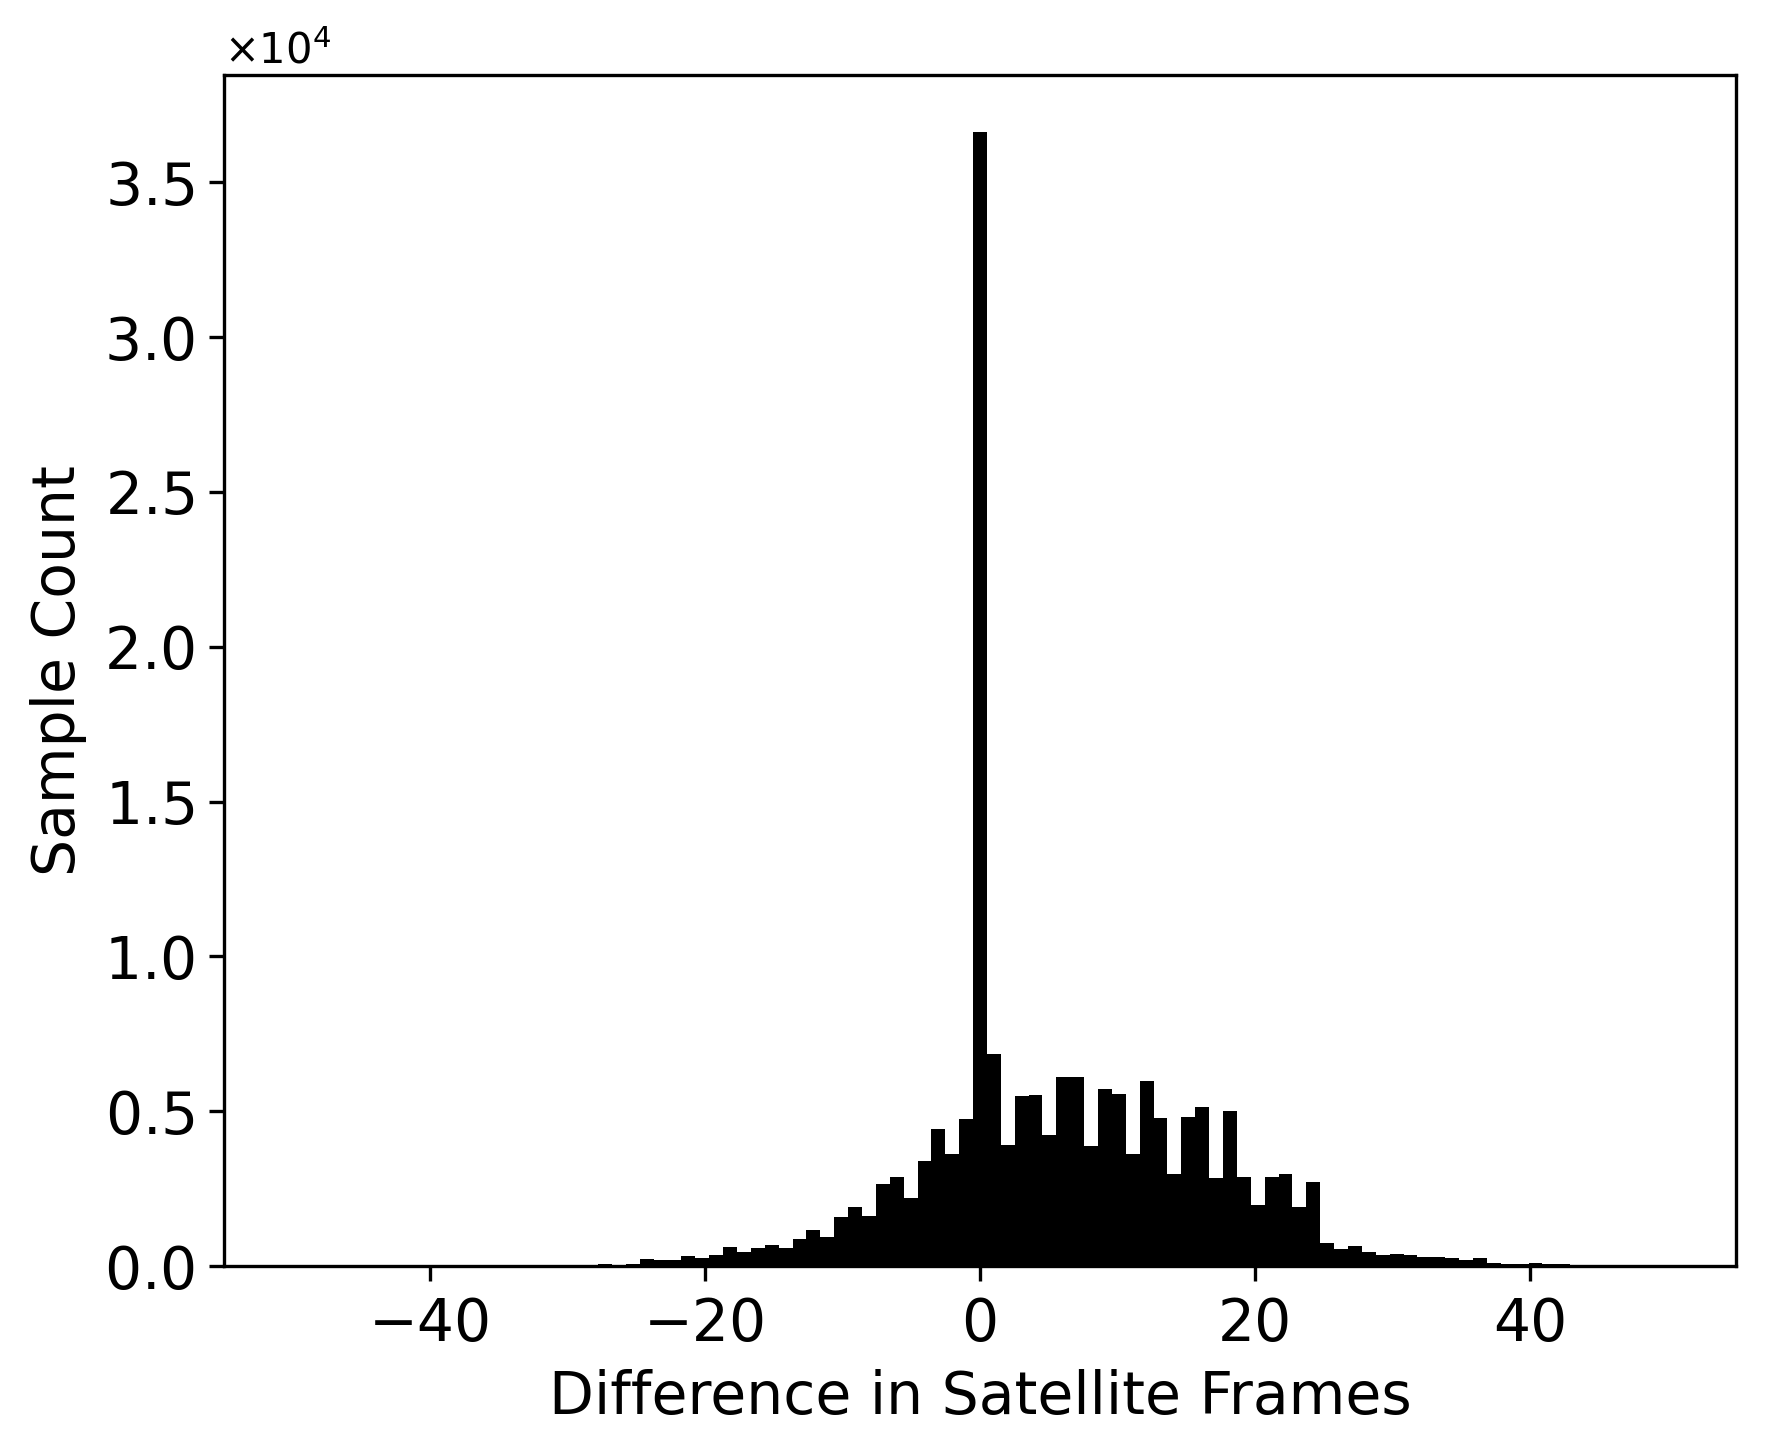
\includegraphics[width=\linewidth]{stat_figs/sample_count_vs_diff_frames.png}
    \caption{The number of satellite frame difference between the \(\mathcal{D}_M\) satellite image and \(\mathcal{D}_p\) chosen satellite image. GOES Full disk images are generated on 10 minute intervals. The number of samples that use the same satellite image in both datasets was 36,608 (\(\approx\)20\%).}\label{all_bands}
\end{figure}


\begin{figure}[!htb]
    \centering
    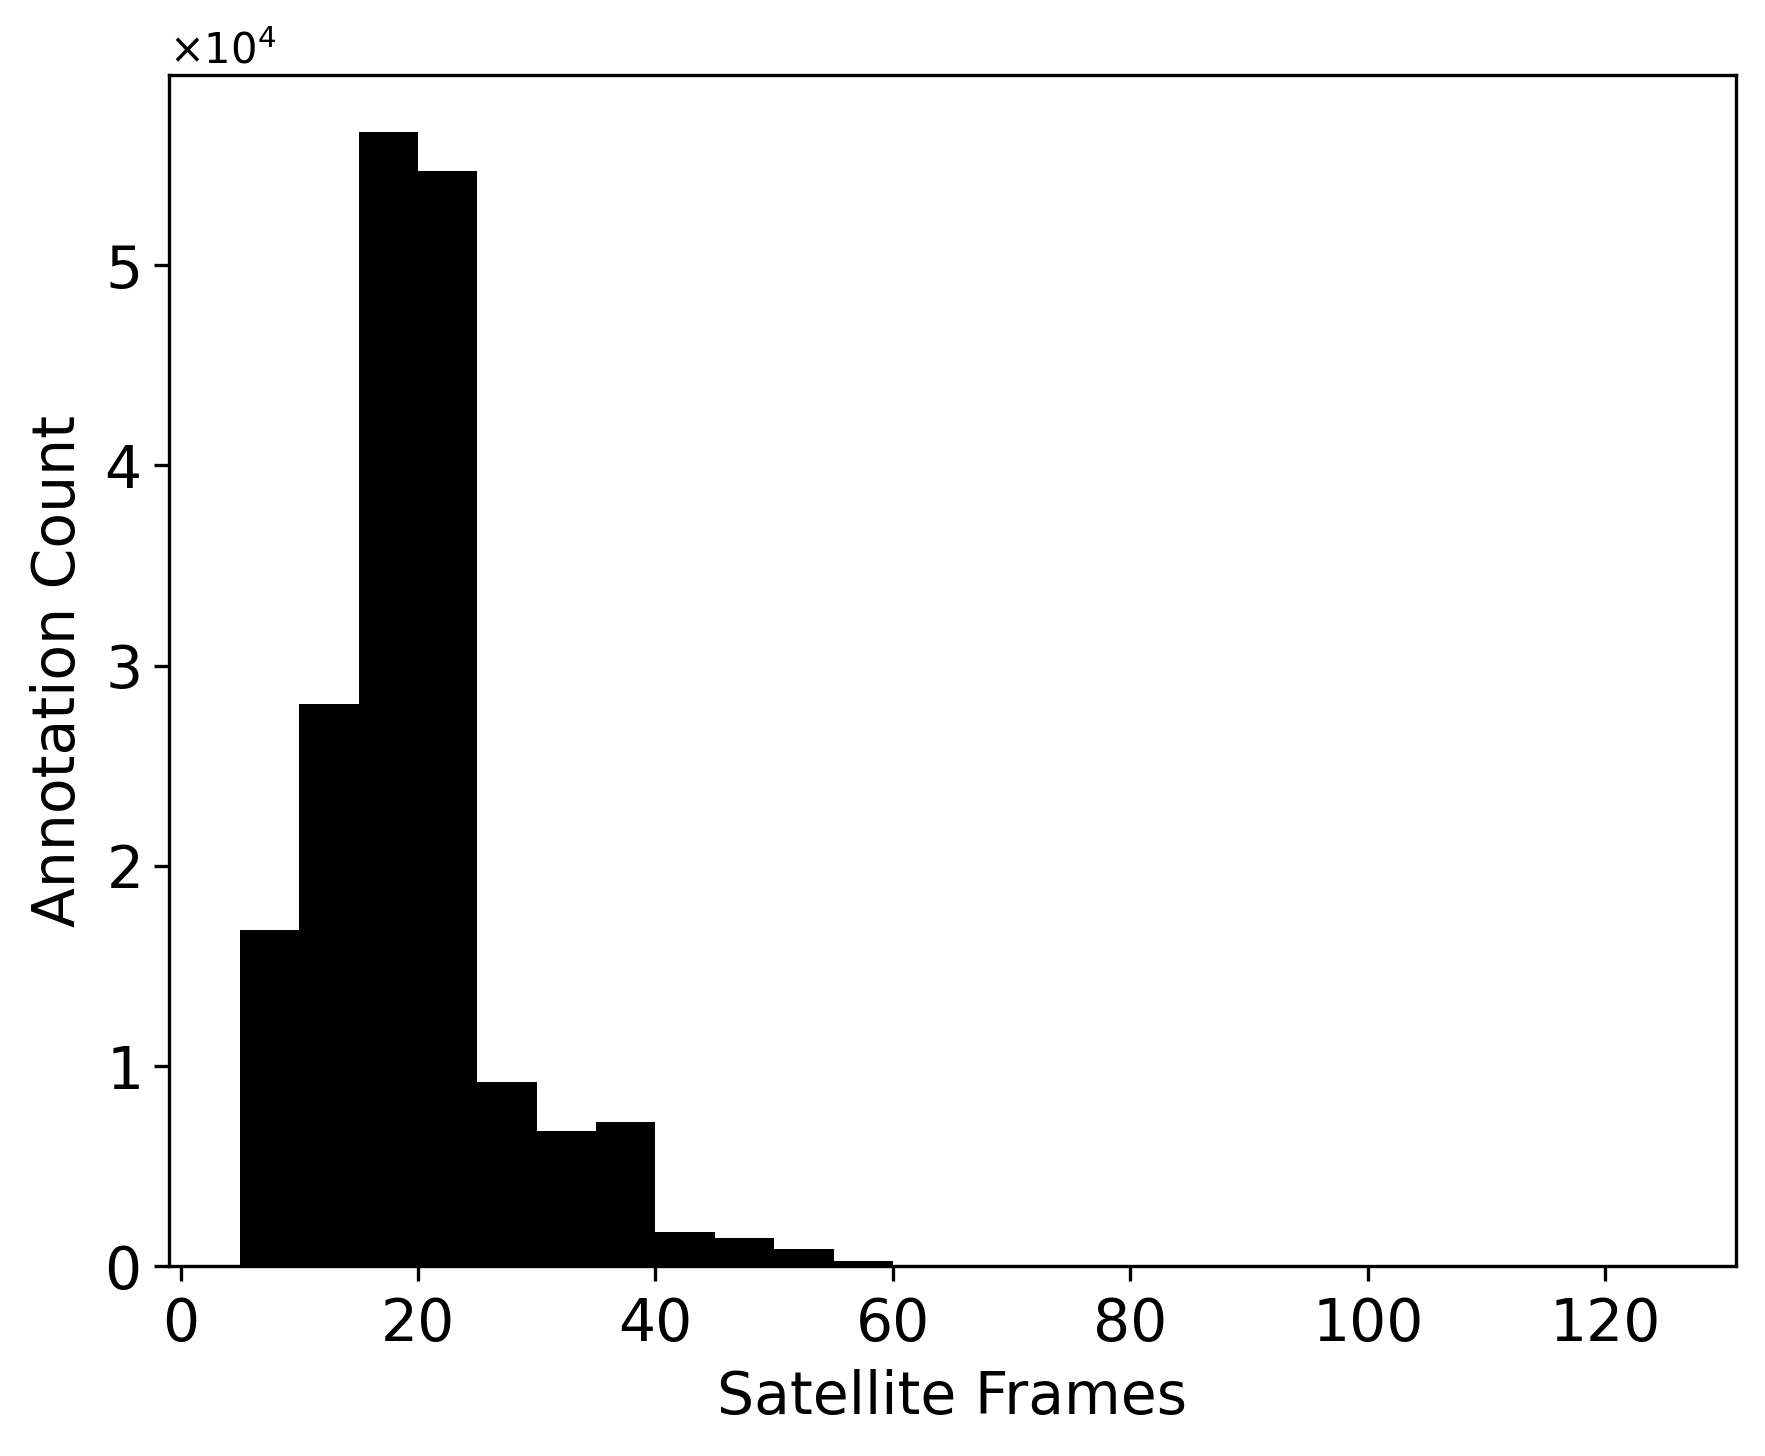
\includegraphics[width=\linewidth]{stat_figs/sample_count_vs_frames.png}
    \caption{The number of annotations that span a number of satellite frames that are generated at a 10-minute interval.}\label{all_bands}
\end{figure}

\begin{figure}[!htb]
    \centering
    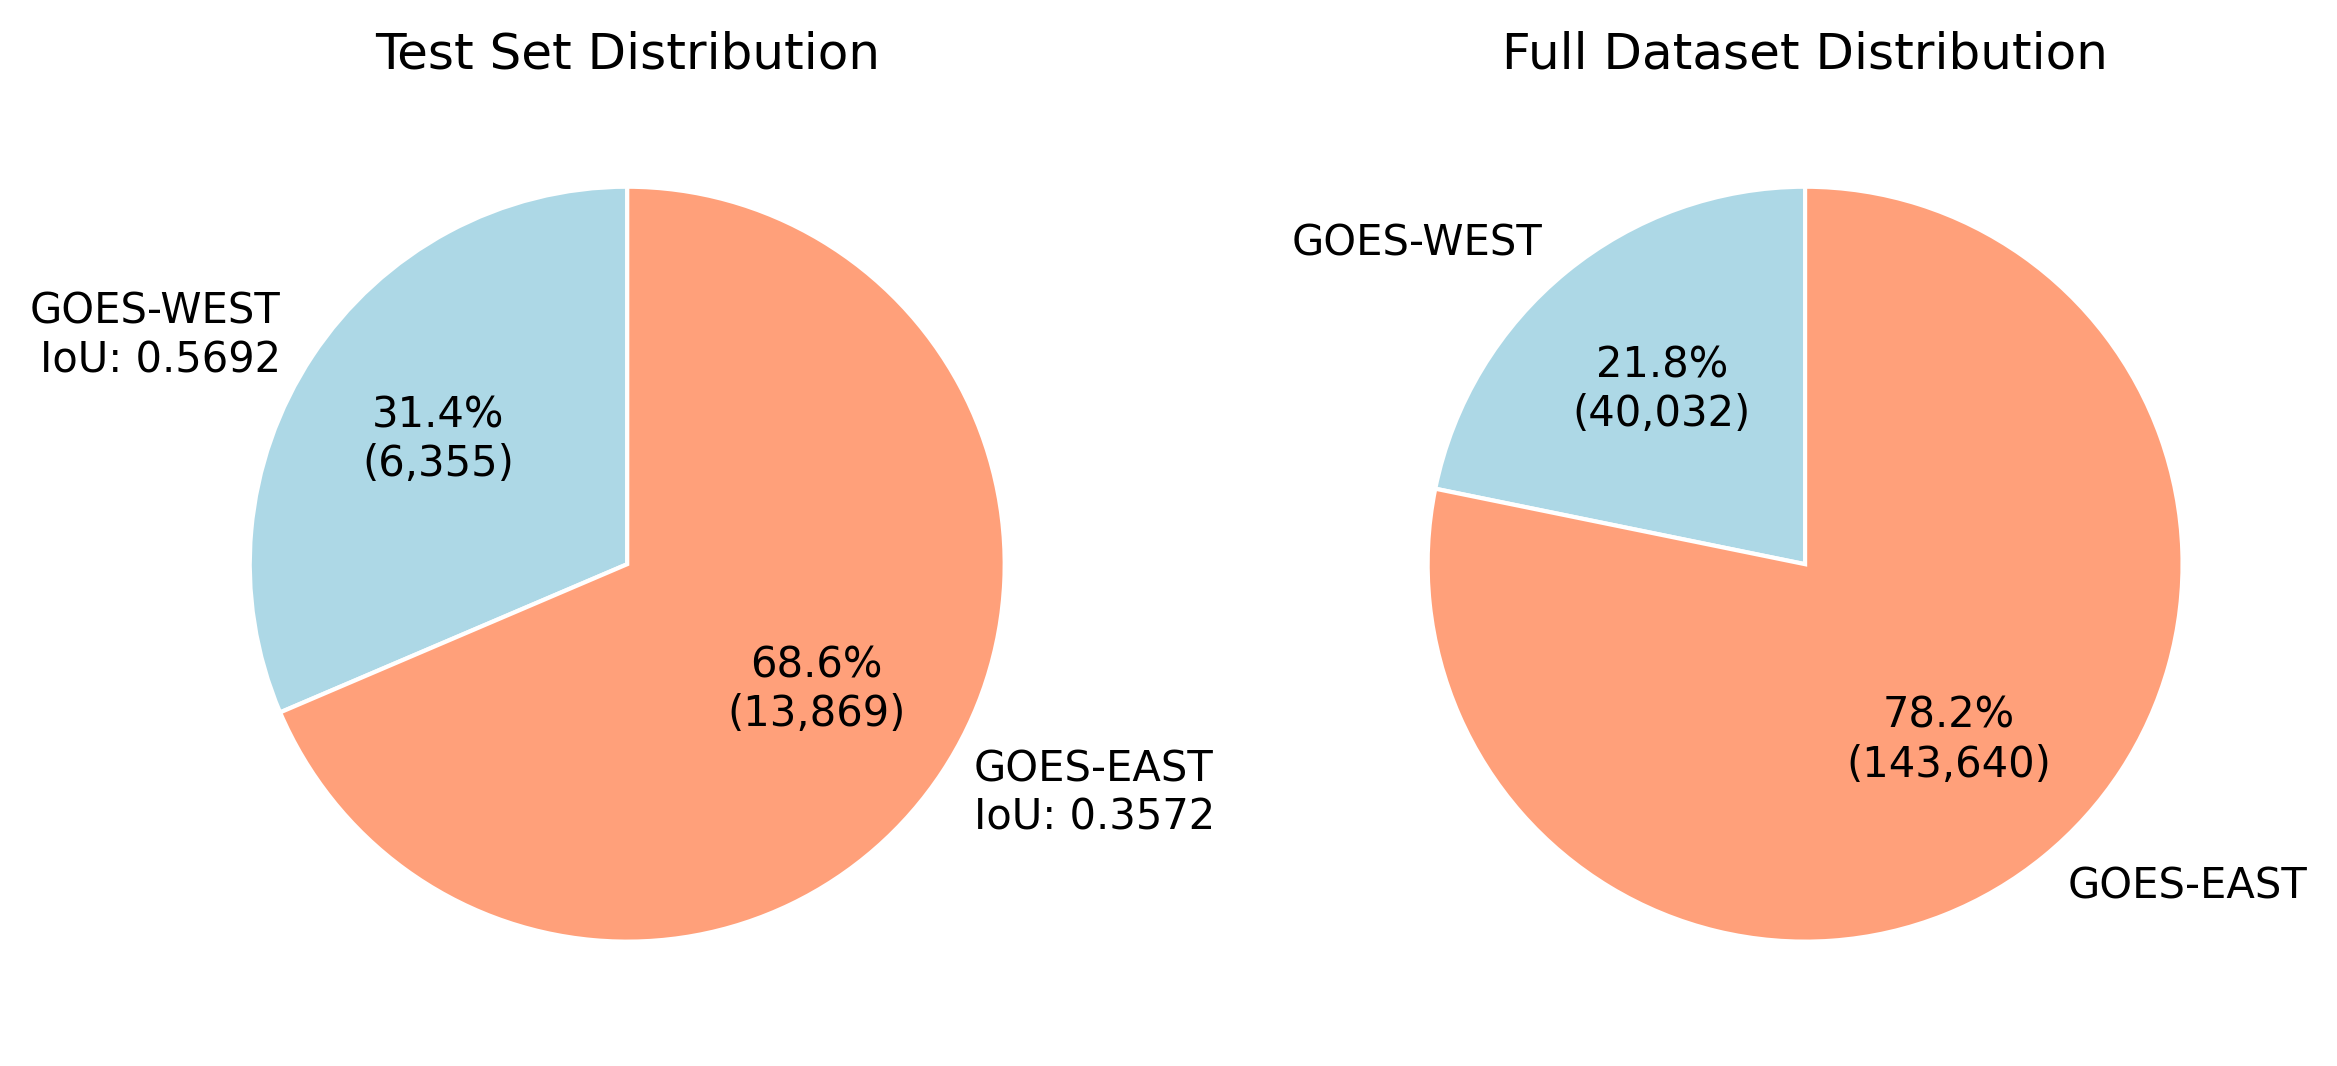
\includegraphics[width=\linewidth]{stat_figs/satellite_test_full_dataset.png}
    \caption{The SmokeViz test set (left) and full SmokeViz dataset (right) distributions by observational satellite.}\label{all_bands}
\end{figure}

\subsection{Model Performance Analysis}

In order to get a better understanding of the dataset, we use the deep learning models to analyze certain data characteristics. Figure \ref{count_per_month} shows variations in overall IoU values running \(f_{c}\) on the \(\mathcal{D}_p\) test set data. The highest IoU are during the typical wildfire season and outside the typical window for prescribed agricultural burns. 

We report on how many samples come from each satellite in table \ref{sample_count_sat}, along with the \(\mathcal{D}_p\) test set IoU in comparison to the HMS analyst annotations. While GOES-EAST provides over triple the number of training samples, \(f_c\) performs better on GOES-WEST samples out of the test set. The signal observed by a single satellite vary diurnally and annually in the amount of atmospheric noise and solar radiation. In turn, if provided with enough samples, this could create a more robust and generalizable model to the extent of being able to perform well on two different sensors with varying calibrations and line of sights. 

As mentioned in the limitations, there may have been a bias introduced towards correctly classifying imagery close to sunrise or sunset. This bias may not only be introduced by our Mie-derived dataset that was used to train \(f_{\circ}\), but also in the original HMS annotations. The configuration of the sun, smoke and satellite give the highest signal-to-noise ratio at the times near the sunrise and sunset, making smoke more easily observable. In contrast, the diurnal variations of wildfires cause the fire radiative power to be highest around solar noon \cite{diurnal}. Table \ref{two_hr_iou} shows how the IoU between \(f_c\) predictions and analyst annotations for the test data from either \(\mathcal{D}_M\) or \(\mathcal{D}_p\) vary based on proximity to sunset/sunrise. One explanation for better values for midday samples could be due to higher amounts of fire activity midday and higher amounts of atmospheric interaction noise early/late in the day. Another difference we see from table \ref{two_hr_iou} is the split of closer to daylight boundaries is shifted towards midday between \(\mathcal{D}_M\) to \(\mathcal{D}_p\). This is because, for \(\mathcal{D}_p\), we are choosing the imagery with the best overlap to the analyst product rather than the image from \(\mathcal{D}_M\) that optimized for highest possible signal-to-noise ratio if given constant signal.

In order to observe geographical regional variations we create quadrants, Northwest (NW), Southwest (SW), Northeast (NE) and Southeast (SE) in relation to the midpoint (40, -105) and show the sample distribution and model performance for each region in table \ref{quad}. The table shows the worst \(f_c\) performance in the SE quadrant despite representing this largest fraction of the training data. This is likely due to the large number of aforementioned prescribed burns in that area. If the goal of the dataset is to be used to train a model to detect and monitor large wildfires, a weakness in the dataset would be that it likely consists of a lot more small, controlled agricultural burns that aren't representative of the intended task. 


\begin{table}
    \caption{Sample count along with variations in \(f_c\) performance depending on which GOES satellite data is used.}
  \label{sample_count_sat}
  \centering
  \begin{tabular}{llll}
    \toprule
    Satellite & Test IoU & \(\mathcal{D}_p\) Test Samples & \(\mathcal{D}_p\) Samples \\
    \midrule
    GOES-WEST & 0.5692 & 6355 & 40032\\
    GOES-EAST & 0.3572 & 13869 & 143640\\
    \bottomrule
  \end{tabular}
\end{table}


\begin{table*}
    \caption{Variations in \(f_c\) performance depending on temporal proximity to sunrise or sunset.}
  \label{two_hr_iou}
  \centering
  \begin{tabular}{lllll}
    \toprule
    Time difference & \(\mathcal{D}_M\) Test Set IoU & \(\mathcal{D}_p\) Test Set IoU & \(\mathcal{D}_M\) Test Samples & \(\mathcal{D}_p\) Test Samples \\ 
    \midrule
    \(<2\) hours & 0.389 & 0.578 & 14100 (65\%) & 8906 (46\%)\\
    \(>2\) hours & 0.492 & 0.606 & 7441 (35\%) &  11318 (54\%) \\
    \bottomrule
  \end{tabular}
\end{table*}


\begin{table}
    \caption{Along with sample count we show variations in \(f_{c}\) performance depending on quadrant.}
  \label{quad}
  \centering
  \begin{tabular}{llll}
    \toprule
    Quadrant & \(\mathcal{D}_p\) Test IoU & \(\mathcal{D}_p\) Test Samples & \(\mathcal{D}_p\) Samples \\
    \midrule
    NW & 0.6418 & 4177 & 32792\\
    SW & 0.6070 & 1937 & 34267\\
    NE & 0.6811 & 1133   & 13342\\
    SE & 0.5581 & 12977 & 103271 \\
    \bottomrule
  \end{tabular}
\end{table}

\subsection{Qualitative Analysis on Performance}

Figure \ref{poor} gives some examples of when SmokeViz does not perform well in comparison to the HMS analyst annotations. In the first column example, SmokeViz confuses a smoke-like cloud for smoke, something it generally tends to not seem to have issues with, but this is an counter example to that trend. The second through last columns all miss distinctive plumes that should be classified as either medium or heavy density smoke. In contrast, we show what SmokeViz looks like when it performs well in comparison to the HMS smoke product in figure \ref{good}.

\begin{figure}[!htb]
    \centering
    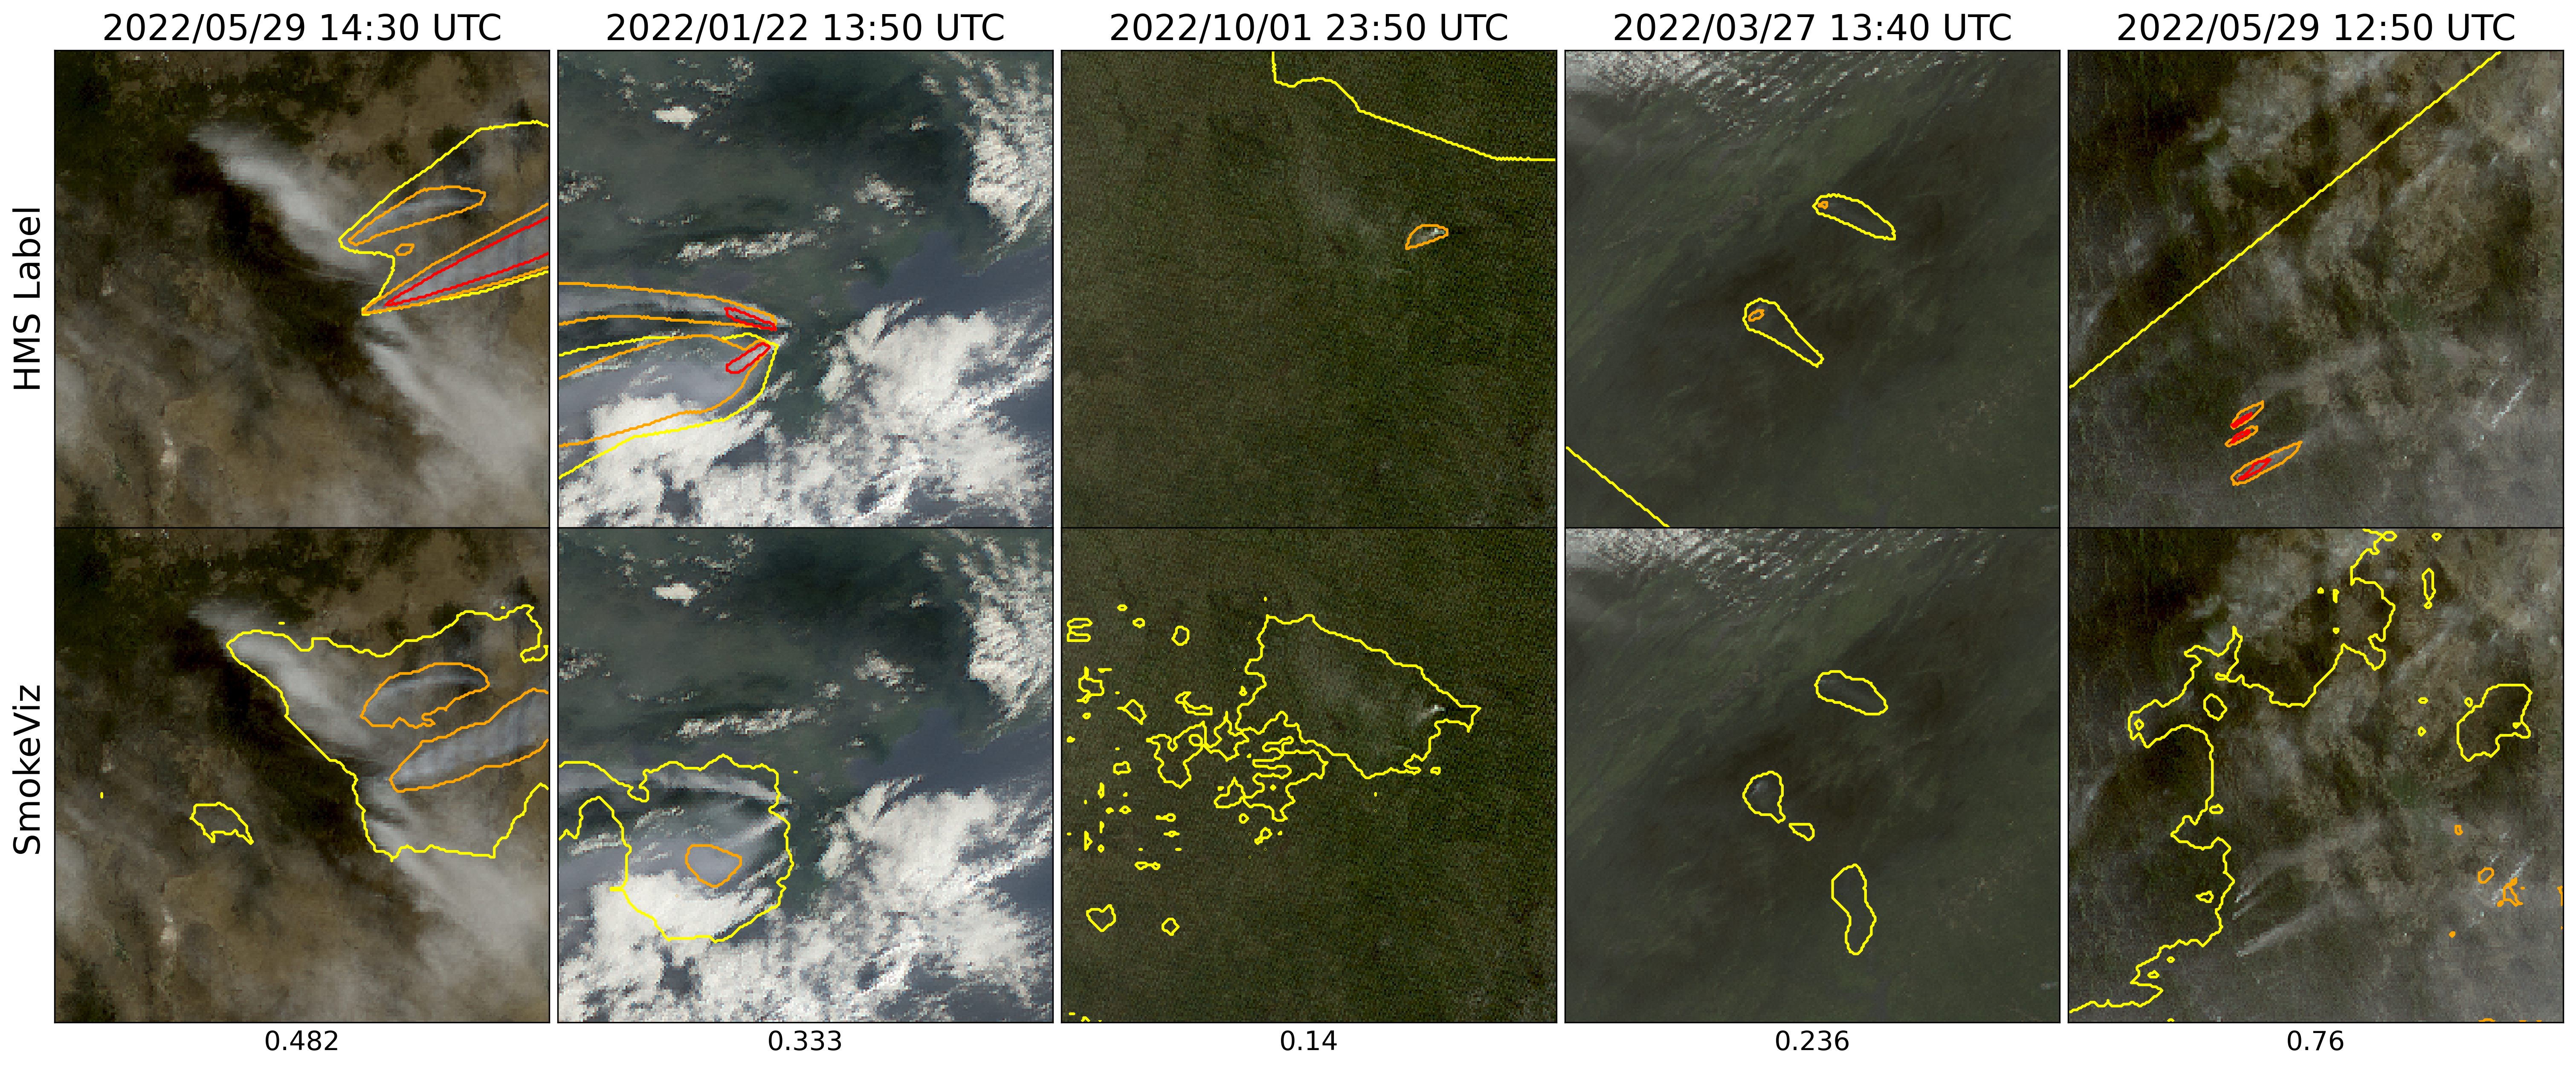
\includegraphics[width=\linewidth]{stat_figs/bad_results.png}
    \caption{Examples of Smoke Viz performing poorly.}
    \label{poor}
\end{figure}


\begin{figure}[!htb]
    \centering
    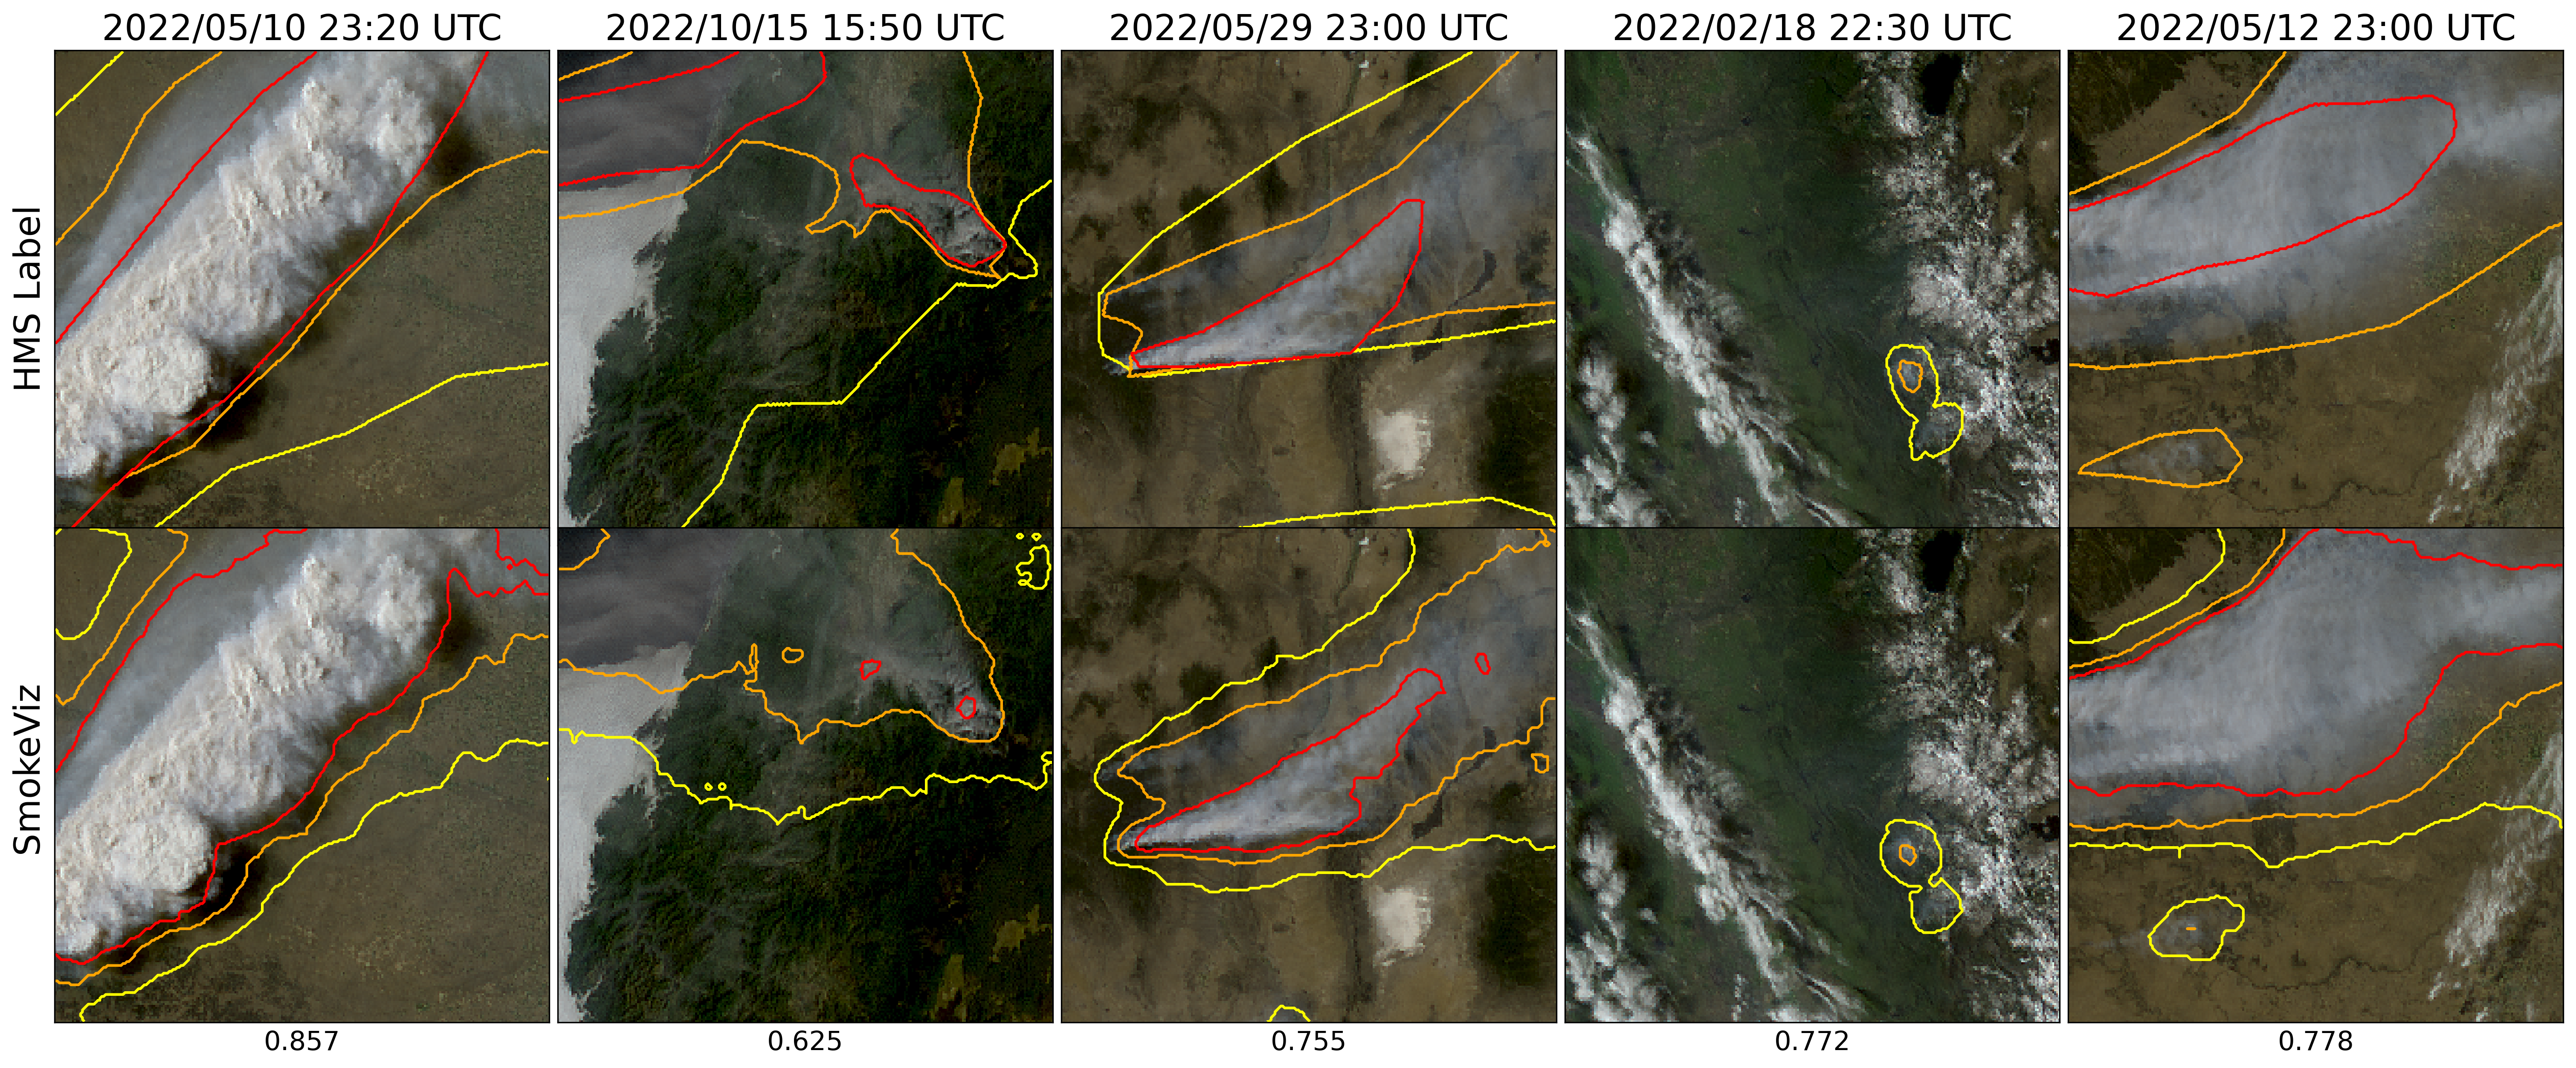
\includegraphics[width=\linewidth]{stat_figs/good_results.png}
    \caption{Examples of Smoke Viz performing well.}
    \label{good}
\end{figure}


\subsection{Machine Learning Reproducibility}

All relevant code is accessible at \url{https://github.com/anonymous-smokeviz/SmokeViz}. The models presented in this paper are not optimized for performance, but are intended to create sufficient pseudo-labels to develop the SmokeViz dataset and then compare the performance of SmokeViz against the original dataset. Due to limited computational resources, we did not perform experimentation for deciding on architecture or hyperparameters shown in table \ref{hyper}, but did make educated decisions. We chose DeepLabV3+ because smoke varies in scale and the DeepLabV3+ backbone uses a atrous spatial pyramid pooling module that allows for varying scales of the same type of object. We use the Adam optimizer that will adapt the learning rate during training and is suited for problems with large amounts of data. Batch size was chosen due to the necessity to run the model on limited resources. 

\begin{table}
    \caption{Hyperparameters used to create \(f_{\circ}\) and \(f_{c}\).}
  \label{hyper}
  \centering
  \begin{tabular}{ll}
    \toprule
    parameter & value \\ 
    \midrule
    epochs & 100 \\
    learning rate & 1e-4 \\
    batch size & 16 \\
    optimizer & Adam \\
    \bottomrule
  \end{tabular}
\end{table}


\pagebreak

\subsection{Datasheet for SmokeViz}

Questions from the https://arxiv.org/abs/1803.09010 paper, v7.

\subsubsection{Motivation}

The questions in this section are primarily intended to encourage dataset creators to clearly articulate their reasons for creating the dataset and to promote transparencyabout funding interests.

\textbf{For what purpose was the dataset created? }

SmokeViz was created to serve as a large labeled dataset to be used in creating wildfire smoke plume related machine learning models. Applications include wildfire smoke detection or smoke dispersion modeling.

\textbf{Who created the dataset (e.g., which team, research group) and on behalf of which entity (e.g., company, institution, organization)?}

REMOVED TO KEEP ANONYMITY DURING REVIEW PROCESS.

\textbf{Who funded the creation of the dataset?} 

REMOVED TO KEEP ANONYMITY DURING REVIEW PROCESS.

\textbf{Any other comments?}

None.

\subsubsection{Composition}

Most of these questions are intended to provide dataset consumers with the information they need to make informed decisions about using the dataset for specific tasks. The answers to some of these questions reveal information about compliance with the EU’s General Data Protection Regulation (GDPR) or comparable regulations in other jurisdictions.

\textbf{What do the instances that comprise the dataset represent (e.g., documents, photos, people, countries)?}

Each instance is a 256x256x3 RGB image from GOES imagery with an accompanying 256x256x3 binary masks corresponding to density of smoke. There are 3 densities of smoke - Light, Medium and Heavy.


\textbf{How many instances are there in total (of each type, if appropriate)?} 

There are 183,672 samples - 128,755 for light, 35,710 for medium and 19,207 for heavy density smoke.


\textbf{Does the dataset contain all possible instances or is it a sample (not necessarily random) of instances from a larger set? }

The entire possible number of samples between 2018/01/01 - 2024/11/01 is 210,702. The dataset is reduced to 207,106 samples after filtering out any samples with no corresponding satellite imagery available or imagery that is less than 10 or over 90 percent saturation. Total saturation is defined when each pixel is equal to 1. Mentioned in more detail in the paper, the dataset was further reduced down to 183,672 samples after applying a .01 IoU threshold during the pseudo-labeling process.

\textbf{What data does each instance consist of? }

The data is processed to correct for Rayleigh scattering, solar zenith angle and projected so each pixel is representative of the same area of land. The algorithm is referenced in the SmokeViz paper.

\textbf{Is there a label or target associated with each instance?}

Yes, there are no samples that are intended to not display any smoke.

\textbf{Is any information missing from individual instances?}

We have seen imagery where smoke is labeled but there's adjacent smoke plumes that were unlabeled. With human labels comes human errors.

\textbf{Are relationships between individual instances made explicit (e.g., users’ movie ratings, social network links)?}

Some instances can overap in geographic location, there can be multiple smoke plumes in one instance, but the index of the HMS smoke annotation is listed and can be mapped back to the original dataset for geolocational information.

\textbf{Are there recommended data splits (e.g., training, development/validation, testing)?}

We recommend using full years of data for training, validation and testing to keep full year long patterns of wildfire behavior. We use 2018-2021 and 2024 for training, 2023 for validation and 2022 for testing.

\textbf{Are there any errors, sources of noise, or redundancies in the dataset?}

The HMS smoke annotations that are used as truth are a source of noise as explained in the SmokeViz paper. These include approximations of smoke polygons mismatching actual location and time windows being too large that smoke moves during the time window. There is also noise caused by atmospheric interactions with light. Redundancies occur when there more than one smoke plume and annotation in one image.

\textbf{Is the dataset self-contained, or does it link to or otherwise rely on external resources (e.g., websites, tweets, other datasets)?}

The dataset is self-contained.

\textbf{Does the dataset contain data that might be considered confidential (e.g., data that is protected by legal privilege or by doctor-patient confidentiality, data that includes the content of individuals’ non-public communications)?}

No.

\textbf{Does the dataset contain data that, if viewed directly, might be offensive, insulting, threatening, or might otherwise cause anxiety?}

No.

\textbf{Does the dataset relate to people? }

No, not directly, although wildfires do affect people, these images are at 1km resolution and do not show enough detail to relate to people or infrastructure.

\textbf{Does the dataset identify any subpopulations (e.g., by age, gender)?}

No.

\textbf{Is it possible to identify individuals (i.e., one or more natural persons), either directly or indirectly (i.e., in combination with other data) from the dataset?}

No.

\textbf{Does the dataset contain data that might be considered sensitive in any way (e.g., data that reveals racial or ethnic origins, sexual orientations, religious beliefs, political opinions or union memberships, or locations; financial or health data; biometric or genetic data; forms of government identification, such as social security numbers; criminal history)?}

No.

\textbf{Any other comments?}

No.


\subsubsection{Collection process}

The answers to questions here may provide information that allow others to reconstruct the dataset without access to it.

\textbf{How was the data associated with each instance acquired?}

The labels from HMS smoke product are not validated or verified but is used for AirNow air quality assessments. The GOES imagery is collected by the ABI sensor and is corrected for any anomalies and also converted from photon count to radiance values.

\textbf{What mechanisms or procedures were used to collect the data (e.g., hardware apparatus or sensor, manual human curation, software program, software API)?}

Original low temporal resolution annotations were manual human analyst curated. To create the high temporal resolution annotations, we use pseudo-labeling discussed in detail within the SmokeViz paper.

\textbf{If the dataset is a sample from a larger set, what was the sampling strategy (e.g., deterministic, probabilistic with specific sampling probabilities)?}

The HMS smoke analysts are only looking for smoke during the daytime and do avoid annotations during heavy cloud cover.

\textbf{Who was involved in the data collection process (e.g., students, crowdworkers, contractors) and how were they compensated (e.g., how much were crowdworkers paid)?}

The NOAA NESDIS employed analysts are compensated as salaried federal employees.

\textbf{Over what timeframe was the data collected?}

2018-2024

\textbf{Were any ethical review processes conducted (e.g., by an institutional review board)?}

No.


\subsubsection{Preprocessing/cleaning/labeling}


The questions in this section are intended to provide dataset consumers with the information they need to determine whether the “raw” data has been processed in ways that are compatible with their chosen tasks. For example, text that has been converted into a “bag-of-words” is not suitable for tasks involving word order.

\textbf{Was any preprocessing/cleaning/labeling of the data done (e.g., discretization or bucketing, tokenization, part-of-speech tagging, SIFT feature extraction, removal of instances, processing of missing values)?}

The data was processed according to the GOES True Color paper referenced in the SmokeViz methods section. This includes atmospheric, Rayleigh corrections and estimation of a Green band.

\textbf{Was the “raw” data saved in addition to the preprocessed/cleaned/labeled data (e.g., to support unanticipated future uses)?}

The raw data is available from the NOAA AWS webpage.
https://registry.opendata.aws/noaa-goes/
The HMS smoke annotations are available here:
https://www.ospo.noaa.gov/products/land/hms.html

\textbf{Is the software used to preprocess/clean/label the instances available?}


Yes, Pytroll implements the algorithm discussed in the GOES True Color paper referenced in the SmokeViz paper.

\textbf{Any other comments?}
None.

\subsubsection{Uses}

These questions are intended to encourage dataset creators to reflect on the tasks for which the dataset should and should not be used. By explicitly highlighting these tasks, dataset creators can help dataset consumers to make informed decisions, thereby avoiding potential risks or harms.

\textbf{Has the dataset been used for any tasks already?}

It was used to train benchmark models mentioned in the paper that apply semantic segmentation to identify and classify smoke in satellite imagery.

\textbf{Is there a repository that links to any or all papers or systems that use the dataset?}

No.

\textbf{What (other) tasks could the dataset be used for?}

A machine learning based smoke dispersion model, automated wildfire smoke detection, create a model that will output a smoke analysis product for data assimilation into smoke or air quality models.

\textbf{Is there anything about the composition of the dataset or the way it was collected and preprocessed/cleaned/labeled that might impact future uses?}

No.

\textbf{Are there tasks for which the dataset should not be used?}

No.
\textbf{Any other comments?}
None

\subsubsection{Distribution}

\textbf{Will the dataset be distributed to third parties outside of the entity (e.g., company, institution, organization) on behalf of which the dataset was created? }

No.

\textbf{How will the dataset will be distributed (e.g., tarball on website, API, GitHub)?}

REMOVED TO KEEP ANONYMITY DURING REVIEW PROCESS.

\textbf{When will the dataset be distributed?}

It is currently available.

\textbf{Will the dataset be distributed under a copyright or other intellectual property (IP) license, and/or under applicable terms of use (ToU)?}

No.

\textbf{Have any third parties imposed IP-based or other restrictions on the data associated with the instances?}

No.

\textbf{Do any export controls or other regulatory restrictions apply to the dataset or to individual instances?}

No.

\textbf{Any other comments?}

None.

\subsubsection{Maintenance}

These questions are intended to encourage dataset creators to plan for dataset maintenance
and communicate this plan with dataset consumers.

\textbf{Who is supporting/hosting/maintaining the dataset?}

REMOVED TO KEEP ANONYMITY DURING REVIEW PROCESS.

\textbf{How can the owner/curator/manager of the dataset be contacted (e.g., email address)?}

REMOVED TO KEEP ANONYMITY DURING REVIEW PROCESS.

\textbf{Is there an erratum?}

No.

\textbf{Will the dataset be updated (e.g., to correct labeling errors, add new instances, delete instances)?}

yes

\textbf{If the dataset relates to people, are there applicable limits on the retention of the data associated with the instances (e.g., were individuals in question told that their data would be retained for a fixed period of time and then deleted)?}

Not applicable.

\textbf{Will older versions of the dataset continue to be supported/hosted/maintained?}

No, if it needs to be updated, it is too large to keep multple versions.

\textbf{If others want to extend/augment/build on/contribute to the dataset, is there a mechanism for them to do so?}

We encourage anyone that would like to contribute to SmokeViz to reach out to REMOVED TO KEEP ANONYMITY DURING REVIEW PROCESS.

\textbf{Any other comments?}

None


\end{document}
